% !TeX spellcheck = pt_PT
\documentclass[12pt,a4paper]{article}
\usepackage[portuguese]{babel}
\usepackage[utf8]{inputenc} 
\usepackage{natbib}
\usepackage{graphicx}
\usepackage{listings}
\author{André Cirne e José Sousa}
\title{Aprendizagem máquina e o ID3}
\begin{document}
	
\begin{titlepage}
	\centering
	{\scshape\LARGE Faculdade de Ciências \par}
	\vspace{1cm}
	{\scshape\Large Inteligência Artificial\par}
	\vspace{1.5cm}
	{\huge\bfseries Trabalho 4\par}
	\vspace{2cm}
	{\Large\itshape André Cirne e José Sousa\par}
	\vfill
	
	{\large \today\par}
\end{titlepage}

\tableofcontents

\section{Introdução}
Uma árvore de decisão é a representação de uma função que efetua a avaliação a um determinado conjunto de dados e que consegue retornar uma decisão \cite{stuart2016artificial}, com base em conhecimento que foi previamente dado à máquina. Este tipo de representação de dados é aquele que permite uma mais simples e maior taxa de sucesso quando utilizados em conjunção com algoritmos de indução em árvores de decisão.
Numa árvore de decisão cada nó representa um teste ao conjunto de dados que se pretende avaliar e cada um dos seus ramos encontra-se identificado com os possíveis valores que pode tomar. Estes testes e os seus ramos vão conduzindo o algoritmo até a um nó folha aonde se encontra o valor a ser retornado pela função, que será a sua decisão.

\section{Algoritmos de indução de árvores de decisão}
As árvores de decisão são apenas uma estrutura de dados, logo sem algoritmos capazes de construir estes modelos de previsão de forma eficiente, elas não servem para nada.
Os algoritmos de indução de árvores de decisão são algoritmos que dados o conjunto de dados de exemplo consegue representar de forma genérica as relações existentes entre dados de input e os resultados.Que caso especifico usando essas relações constroem de forma automática a árvore de decisão.\cite{rokach2005top} Estes algoritmos por norma têm uma construção aplicando princípios \textit{greedy} e construido a árvore na direção raiz para as folhas de forma recursiva.
Como o referido anteriormente este algoritmos são de sua essência greedy logo para que em cada nó ele possa efetuar a melhor escolha vai utilizar métricas.
\subsection{Métricas}
\subsubsection{Ganho de informação}
O ganho de informação é baseado no conceito de entropia.
A entropia é a media de incerteza que há num sistema. Usando o conceito de entropia podemos calcular a probabilidade de ocorrência de um determinado evento em cada conjunto de resultados.
Dado um conjunto S, com instâncias pertencentes à classe i, com probabilidade  $\phi$, temos:

\begin{equation}
	Entropia = \sum_{i=0}^{i} \phi\log\phi
\end{equation}

\subsubsection{Impuridade de Gini}
A impuridade Gini é uma métrica que mede a divergência entre a distribuição probabilística  dos valores que atributo toma.  

\subsection{ID3}
O algoritmo ID3 (inductive decision tree) é um dos mais utilizados para a construção de árvores de decisão. Este algoritmo tem como objetivo a construção de uma árvore de decisão que explique cada instância de um sequencia de entrada, da maneira mais compacta. Em cada momento elege o melhor atributo dependendo de uma determinada heurística.  
O ID3 segue os seguintes passos:
\begin{enumerate}
	\item 	Começar com todos os exemplos de treino;
	\item	Escolher o teste (atributo) que melhor divide os exemplos, ou seja agrupar exemplos da mesma classe ou exemplos semelhantes;
	\item	Para o atributo escolhido, criar um nó filho para cada valor possível do atributo;
	\item	Transportar os exemplos para cada filho tendo em conta o valor do filho;
	\item	Repetir o procedimento para cada filho não "puro". Um filho é puro quando cada atributo X tem o mesmo valor em todos os exemplos. 
\end{enumerate}
Mesmo assim deixamos a pensar como é que vamos escolher o nosso melhor atributo?  A resposta esta em dois conceitos: Entropia e Ganho
\subsection{CART}
CART que significa "Classification and Regression Trees" é um algoritmo caracterizado pela construção de árvores de decisão binárias.\cite{rokach2005top} É um algoritmo que não só constrói árvores de classificação mas sim também árvores de regressão, dependendo se a variável em questão é categórica ou numérica.Como métrica para o ganho utiliza a impuridade de gini.
O algoritmo segue as seguinte regras para a construção de árvores de decisão:
\begin{enumerate}
	\item Os valores das variáveis são escolhidos de forma a que divisão seja a melhor a possível.
	\item Logo que a divisão se aplique a este processo é aplicado aos seus filhos.
	\item Esta divisão acaba quando o CART deteta que já não existe nenhum ganho ao fazer a divisão ou no caso da existência de outra regra que ja foi previamente identificada.  
\end{enumerate}

\subsection{C4.5}
O algoritmo C4.5 é um melhoramento do algoritmo ID3, isto devido ao fato de trabalhar com valores indisponíveis, com valores contínuos, podar árvores de decisão e derivar regras.
Trabalhar com atributos que possuem valores indisponíveis na construção de uma árvore da decisão, pode ser considerado um problema. A falta destes valores, pode ocorrer pelo fato de não terem sido registados no momento da recolha dos dados, ou por não serem considerados relevantes para um determinado caso.
Por outras palavra, este algoritmo ignora os valores desconhecidos, ou seja, não utiliza a amostra para os cálculos de entropia e ganho.
Utiliza a medida de razão de ganho para selecionar o melhor atributo que divide os exemplos. Medida superior ao ganho de informação do ID3, gerando árvores menos complexas.

\section{Implementação}
Neste trabalho utilizamos Python 3, devido a ser uma linguagem multi-paradigma e levando assim a uma passagem mais rápida da parte do planeamento para implementação.
A forma como era necessário responder ao problema obrigava-nos a que por um lado conseguíssemos representar e construir de forma organizada uma árvore de decisão capaz não só de armazenar dados brutos mas por exemplo no caso de dados numéricos conseguir agrupá-los de forma a que a árvore se torne mais legível, sem comprometer a fiabilidade da árvore de decisão.  
\subsection{Estrutura de dados}

\subsubsection{Dicionários e listas}


\subsubsection{Leaf}
Estrutura com o objetivo de representar os nós folhas na árvore de decisão. Aqui estará armazenado a resposta ao nó pai, a classe e o contador de casos que se encontram identificados com esta folha.
%\begin{figure}
%	\centering
%	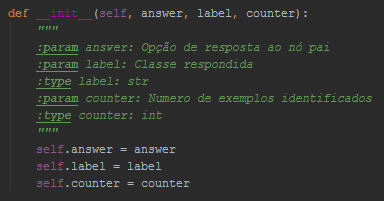
\includegraphics[]{img/leaf.png}
%	\caption{Inicialização da classe leaf.}
%\end{figure}
\subsubsection{Jump}
Estrutura de ser o elo de ligação entre dois nós da árvore  de decisão, a estrutura Jump é composta por um campo answer com a resposta ao nó pai , um contador com o numero de nós que se identificaram com aquele caso e um apontador para outro nó da árvore.
%\begin{figure}
%	\centering
%	\includegraphics[]{img/jump.png}
%	\caption{Inicialização da classe jump.}
%\end{figure}
\subsubsection{Node\_root}
Estrutura que representa cada nó da árvore as suas componentes principais é o atributo e uma lista com todos os deus ramos.
%\begin{figure}
%	\centering
%	\includegraphics[]{img/node.png}
%	\caption{Inicialização da classe Node\_root.}
%\end{figure}

\subsection{Intervalo}
A estrutura intervalo, é aquela que nos permite que consigamos representar intervalos numéricos na árvore de decisão. Da forma como ela foi implementada permite a ordenação de intervalos de forma automática e quando a estrutura intervalo é comprada com um valor numérico se esse se encontrar nos seus limites identifica-o como seu.

\subsection{Organização do código e implementação}
A organização deste código foi feita através da criação de um classe chamada decision tree, ao inicializar esta classe é construida a árvore de decisão utilizando o algoritmo ID3, neste processo de construção também é efetuado a transformação de valores numéricos em intervalos numéricos. No cálculo do ID3 encontramo-nos a utilizar como como heuristica a entropia para decisão de quem vai ser o primeiro argumento a ser escolhido como nó da árvore. É importante referir que no caso de a uma dada altura na construção da árvore existir um ramo que não tenha qualquer~exemplo com o qual possamos atribuir um valor, a este é atribuído o valor mais comum da árvore.
O código tenta trabalhar com base em recursão pelas várias classes.

\subsection{Reflexão}
Durante a fase de já testes do programa chegamos à conclusão que não era necessário ter utilizado a estrutura jump e a estrutura leaf de forma tão complicada já que nos tinha bastado implementar um dicionário onde a \textit{answer} seria a key de pesquisa no dicionário.

\section{Resultados}
\subsection{restaurant.csv}
\begin{lstlisting}
<Pat>
	Some: Yes (4)
	None: No (2)
	Full:
		<Hun>
			No: No (2)
			Yes:
				<Type>
					Italian: No (1)
					Burger: Yes (1)
					Thai:
						<Fri>
							No: No (1)
							Yes: Yes (1)
					French: Yes (0)
\end{lstlisting}

\subsection{weather.csv}
\begin{lstlisting}
<Weather>
	overcast: yes (4)
	sunny:
		<Humidity>
			65.0 <= x < 75.0: yes (2)
			75.0 <= x < 96.1: no (3)
	rainy:
		<Humidity>
			65.0 <= x < 75.0: no (1)
			75.0 <= x < 86.0: yes (2)
			86.0 <= x < 95.0: no (1)
			95.0 <= x < 96.1: yes (1)
\end{lstlisting}

\subsection{iris.csv}
\begin{lstlisting}
<petallength>
	1.0 <= x < 3.0: Iris-setosa (50)
	3.0 <= x < 4.5: Iris-versicolor (29)
	4.5 <= x < 4.7:
		<sepallength>
			4.3 <= x < 4.9: Iris-setosa (0)
			4.9 <= x < 5.0: Iris-virginica (1)
			5.0 <= x < 5.4: Iris-setosa (0)
			5.4 <= x < 5.5: Iris-versicolor (1)
			5.5 <= x < 5.6: Iris-setosa (0)
			5.6 <= x < 5.8: Iris-versicolor (2)
			5.8 <= x < 6.0: Iris-setosa (0)
			6.0 <= x < 6.3: Iris-versicolor (4)
			6.3 <= x < 6.4: Iris-setosa (0)
			6.4 <= x < 6.7: Iris-versicolor (3)
			6.7 <= x < 8.0: Iris-setosa (0)
	4.7 <= x < 4.8: Iris-versicolor (5)
	4.8 <= x < 4.9:
		<sepallength>
			4.3 <= x < 5.9: Iris-setosa (0)
			5.9 <= x < 6.0: Iris-versicolor (1)
			6.0 <= x < 6.1: Iris-virginica (1)
			6.1 <= x < 6.2: Iris-setosa (0)
			6.2 <= x < 6.3: Iris-virginica (1)
			6.3 <= x < 6.8: Iris-setosa (0)
			6.8 <= x < 6.9: Iris-versicolor (1)
			6.9 <= x < 8.0: Iris-setosa (0)
	4.9 <= x < 5.0:
		<sepalwidth>
			2.0 <= x < 2.5: Iris-setosa (0)
			2.5 <= x < 2.6: Iris-versicolor (1)
			2.6 <= x < 2.7: Iris-setosa (0)
			2.7 <= x < 2.9: Iris-virginica (2)
			2.9 <= x < 3.0: Iris-setosa (0)
			3.0 <= x < 3.1: Iris-virginica (1)
			3.1 <= x < 3.2: Iris-versicolor (1)
			3.2 <= x < 4.5: Iris-setosa (0)
	5.0 <= x < 5.1:
		<sepallength>
			4.3 <= x < 5.7: Iris-setosa (0)
			5.7 <= x < 5.8: Iris-virginica (1)
			5.8 <= x < 6.0: Iris-setosa (0)
			6.0 <= x < 6.1: Iris-virginica (1)
			6.1 <= x < 6.3: Iris-setosa (0)
			6.3 <= x < 6.4: Iris-virginica (1)
			6.4 <= x < 6.7: Iris-setosa (0)
			6.7 <= x < 6.8: Iris-versicolor (1)
			6.8 <= x < 8.0: Iris-setosa (0)
	5.1 <= x < 7.0:
		<sepallength>
			4.3 <= x < 5.8: Iris-setosa (0)
			5.8 <= x < 6.0: Iris-virginica (4)
			6.0 <= x < 6.1: Iris-versicolor (1)
			6.1 <= x < 6.6: Iris-virginica (15)
			6.6 <= x < 6.7: Iris-setosa (0)
			6.7 <= x < 8.0: Iris-virginica (22)
\end{lstlisting}

\section{Conclusões}

\bibliographystyle{plain}
\bibliography{bibliografia} 

\end{document}

